\documentclass[a4paper,10pt,twocolumn,oneside]{article}
\setlength{\columnsep}{10pt}                                                              %兩欄模式的間距
\setlength{\columnseprule}{0pt}                                                                %兩欄模式間格線粗細

\usepackage{amsthm}								%定義,例題
\usepackage{amssymb}
%\usepackage[margin=2cm]{geometry}
\usepackage{fontspec}								%設定字體
\usepackage{color}
\usepackage[x11names]{xcolor}
\usepackage{listings}								%顯示code用的
%\usepackage[Glenn]{fncychap}						%排版,頁面模板
\usepackage{fancyhdr}								%設定頁首頁尾
\usepackage{graphicx}								%Graphic
\usepackage{enumerate}
\usepackage{titlesec}
\usepackage{amsmath}
\usepackage{tikz}
\usepackage{xpatch}
\usepackage[CheckSingle, CJKmath]{xeCJK}
% \usepackage{CJKulem}
%\usepackage[T1]{fontenc}
\titlespacing{\section}{0cm}{0cm}{0cm}
\titlespacing{\subsection}{0cm}{0cm}{0cm}
\usepackage{amsmath, courier, listings, fancyhdr, graphicx}
\topmargin=0pt
\headsep=5pt
\textheight=780pt
\footskip=0pt
\voffset=-40pt
\textwidth=545pt
\marginparsep=0pt
\marginparwidth=0pt
\marginparpush=0pt
\oddsidemargin=0pt
\evensidemargin=0pt
\hoffset=-42pt

%\renewcommand\listfigurename{圖目錄}
%\renewcommand\listtablename{表目錄} 

%%%%%%%%%%%%%%%%%%%%%%%%%%%%%


\setmainfont [				%主要字型
    Path = .fonts/ttf/,
    UprightFont = *-Regular,
    BoldFont = *-Bold,
    ItalicFont = *-Italic
  ] {Consolas}

\setmonofont [        
    Path = .fonts/ttf/,
    UprightFont = *-Regular
  ] {Monaco}

% \setmainfont{TeX Gyre Termes}
% \setmainfont{Consolas}				%主要字型
% \setmonofont{Monaco}				%主要字型
\setCJKmainfont{SimSun}

% \setCJKmainfont{Consolas}			%中文字型
% \setmainfont{sourcecodepro}
\XeTeXlinebreaklocale "zh"						%中文自動換行
\XeTeXlinebreakskip = 0pt plus 1pt				%設定段落之間的距離
\setcounter{secnumdepth}{3}						%目錄顯示第三層

%%%%%%%%%%%%%%%%%%%%%%%%%%%%%
\makeatletter
\lst@CCPutMacro\lst@ProcessOther {"2D}{\lst@ttfamily{-{}}{-{}}}
\@empty\z@\@empty
\makeatother
\lstset{											% Code顯示
language=C++,										% the language of the code
basicstyle=\footnotesize\ttfamily, 						% the size of the fonts that are used for the code
%numbers=left,										% where to put the line-numbers
numberstyle=\footnotesize,						% the size of the fonts that are used for the line-numbers
stepnumber=1,										% the step between two line-numbers. If it's 1, each line  will be numbered
numbersep=5pt,										% how far the line-numbers are from the code
backgroundcolor=\color{white},					% choose the background color. You must add \usepackage{color}
showspaces=false,									% show spaces adding particular underscores
showstringspaces=false,							% underline spaces within strings
showtabs=false,									% show tabs within strings adding particular underscores
frame=false,											% adds a frame around the code
tabsize=2,											% sets default tabsize to 2 spaces
captionpos=b,										% sets the caption-position to bottom
breaklines=true,									% sets automatic line breaking
breakatwhitespace=false,							% sets if automatic breaks should only happen at whitespace
escapeinside={\%*}{*)},							% if you want to add a comment within your code
morekeywords={*},									% if you want to add more keywords to the set
keywordstyle=\bfseries\color{Blue1},
commentstyle=\itshape\color{Red4},
stringstyle=\itshape\color{Green4},
}

%%%%%%%%%%%%%%%%%%%%%%%%%%%%%

\begin{document}
\pagestyle{fancy}
\fancyfoot{}
%\fancyfoot[R]{\includegraphics[width=20pt]{ironwood.jpg}}
\fancyhead[L]{NTOU Miaotomata}
\fancyhead[R]{\thepage}
\renewcommand{\headrulewidth}{0.4pt}
\renewcommand{\contentsname}{Contents} 

\newcommand{\includetex}[2]{
  \subsection{#1}
  \input{#2}
  \vspace{-1.2em}
}
\scriptsize
\tableofcontents

% \newpage
%sectionstart
\section{basic}
    \subsection{default}
    \lstinputlisting{basic/default.cpp}

    \subsection{godcode}
    \lstinputlisting{basic/godcode.cpp}

    \subsection{random}
    \lstinputlisting{basic/random.cpp}

    \subsection{run.bat}
    \lstinputlisting{basic/run.bat}

    \subsection{run.sh}
    \lstinputlisting{basic/run.sh}

\section{binarysearch}
    \subsection{二分搜}
    \lstinputlisting{binarysearch/二分搜.cpp}

\section{dataStructure}
    \subsection{DSU}
    \lstinputlisting{dataStructure/DSU.cpp}

    \subsection{fenwickTree}
    \lstinputlisting{dataStructure/fenwickTree.cpp}

    \subsection{segTree}
    \lstinputlisting{dataStructure/segTree.cpp}

\section{dp}
    \subsection{digit}
    \lstinputlisting{dp/digit.cpp}

    \subsection{p\_median}
    \lstinputlisting{dp/p_median.cpp}

    \subsection{sosdp}
    \lstinputlisting{dp/sos_dp.cpp}

\section{flow}
    \subsection{Dinic}
    \lstinputlisting{flow/Dinic.cpp}

    \subsection{isap}
    \lstinputlisting{flow/isap.cpp}

    \subsection{KM}
    \lstinputlisting{flow/KM.cpp}

    \subsection{最小花費最大流dijkstra 不能負值}
    \lstinputlisting{flow/最小花費最大流dijkstra 不能負值.cpp}

    \subsection{最小花費最大流SPFA}
    \lstinputlisting{flow/最小花費最大流SPFA.cpp}

\section{geometry}
    \subsection{basic}
    \lstinputlisting{geometry/basic.cpp}

    \subsection{definition}
    \lstinputlisting{geometry/definition.cpp}
    
    \subsection{complex}
    \lstinputlisting{geometry/complex.cpp}

    \subsection{ConvexHull}
    \lstinputlisting{geometry/ConvexHull.cpp}

    \subsection{MEC}
    \lstinputlisting{geometry/MEC.cpp}

    \subsection{MECrandom}
    \lstinputlisting{geometry/MECrandom.cpp}

    \subsection{Rotating Clipers}
    \lstinputlisting{geometry/rotating.cpp}

    \subsection{sortbyangle}
    \lstinputlisting{geometry/sortbyangle.cpp}

\section{graph}
    \subsection{BCC}
    \lstinputlisting{graph/BCC.cpp}

    \subsection{SCC}
    \lstinputlisting{graph/SCC.cpp}

    \subsection{支配樹}
    \lstinputlisting{graph/支配樹.cpp}

    \subsection{最大團}
    \lstinputlisting{graph/最大團.cpp}

    \subsection{最小圈}
    \lstinputlisting{graph/最小圈.cpp}

\section{math}
    \subsection{DiscreteSqrt}
    \lstinputlisting{math/DiscreteSqrt.cpp}

    \subsection{excrt}
    \lstinputlisting{math/excrt.cpp}

    \subsection{exgcd}
    \lstinputlisting{math/exgcd.cpp}

    \subsection{FFT}
    \lstinputlisting{math/FFT.cpp}

    \subsection{josephus}
    \lstinputlisting{math/josephus.cpp}

    \includetex{Theorem}{math/theorem.tex}
    \vspace{1.2em}
    \includetex{Primes}{math/Primes.tex}
    \vspace{1.2em}
    \subsection{millerrabin}
    \lstinputlisting{math/miller_rabin.cpp}

    \subsection{phi}
    \lstinputlisting{math/phi.cpp}

    \subsection{pollardrho}
    \lstinputlisting{math/pollard_rho.cpp}

    \subsection{primes}
    \lstinputlisting{math/primes.cpp}

    \subsection{Euler}
    \lstinputlisting{math/euler.cpp}

    \subsection{quickeuler}
    \lstinputlisting{math/quick_euler.cpp}

    \subsection{sieve}
    \lstinputlisting{math/sieve.cpp}

\section{string}
    \subsection{KMP}
    \lstinputlisting{string/KMP.cpp}

    \subsection{minRotation}
    \lstinputlisting{string/minRotation.cpp}

    \subsection{PalindromeTree}
    \lstinputlisting{string/PalindromeTree.cpp}

    \subsection{RollingHash}
    \lstinputlisting{string/RollingHash.cpp}

    \subsection{SuffixArray}
    \lstinputlisting{string/SuffixArray.cpp}

    \subsection{trie}
    \lstinputlisting{string/trie.cpp}

    \subsection{Z-algorithm}
    \lstinputlisting{string/Z-algorithm.cpp}

    \subsection{馬拉車}
    \lstinputlisting{string/馬拉車.cpp}

\section{tree}
    \subsection{DSUONTREE}
    \lstinputlisting{tree/DSUONTREE.cpp}

    \subsection{EularTour}
    \lstinputlisting{tree/Eular_Tour.cpp}

    \subsection{LCA}
    \lstinputlisting{tree/LCA.cpp}

    \subsection{treehash}
    \lstinputlisting{tree/tree_hash.cpp}


%sectionend


% 方格紙
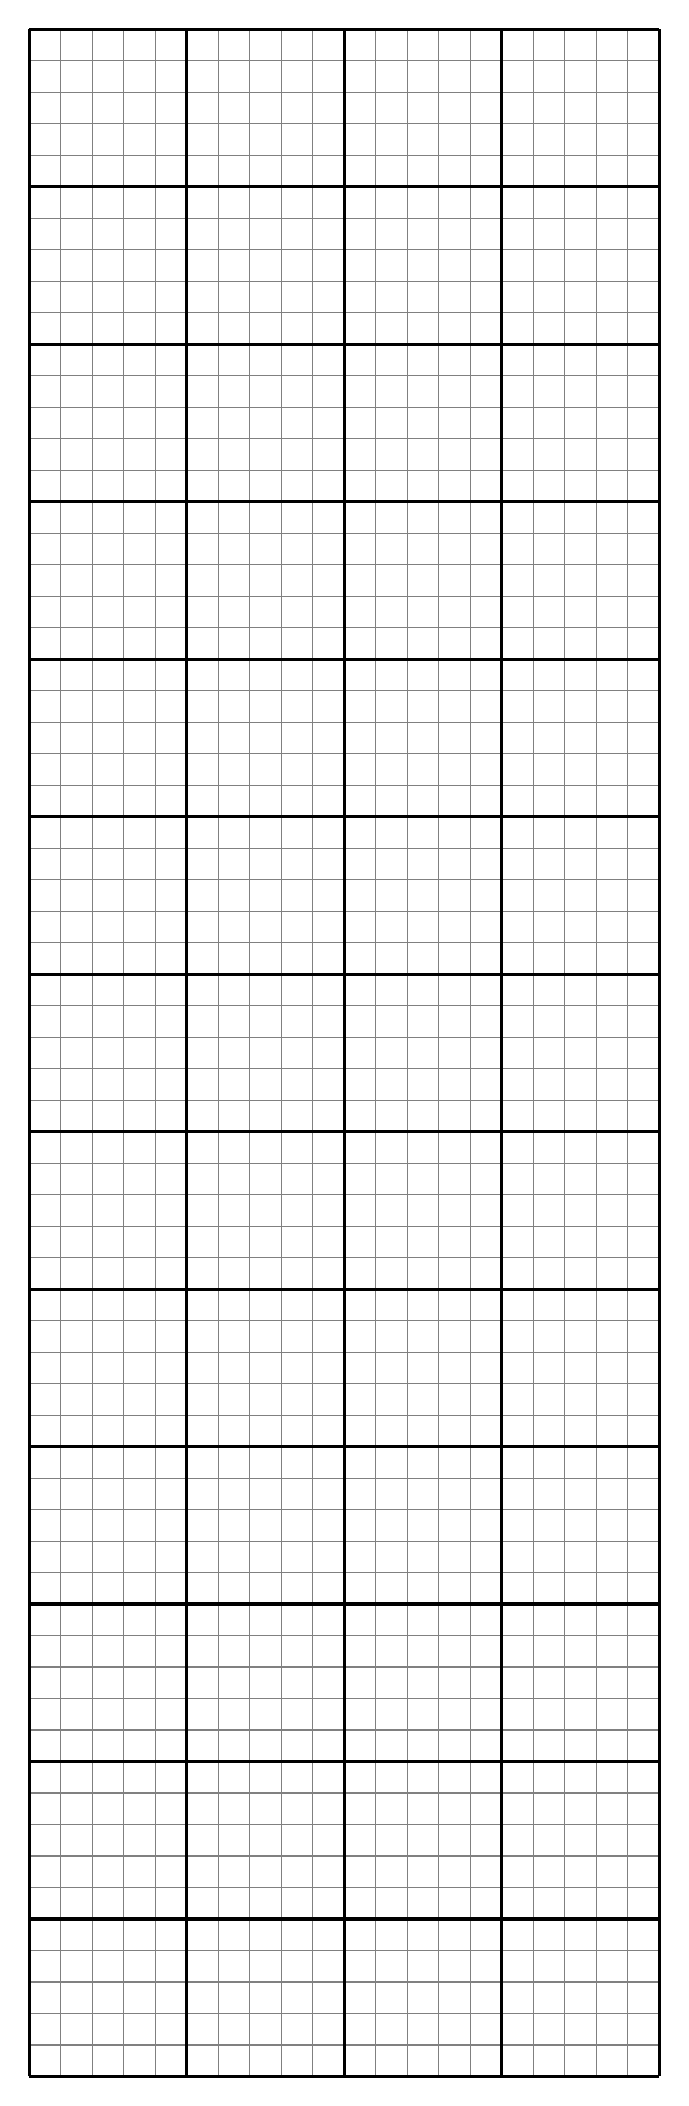
\begin{tikzpicture}[every node/.style={minimum size=1cm-\pgflinewidth, outer sep=10pt}, scale=2]
    \draw[step=0.2cm,color=gray] (0,0) grid (4,13);
    \draw[step=1cm,color=black,line width=0.4mm] (0,0) grid (4,13);
\end{tikzpicture}
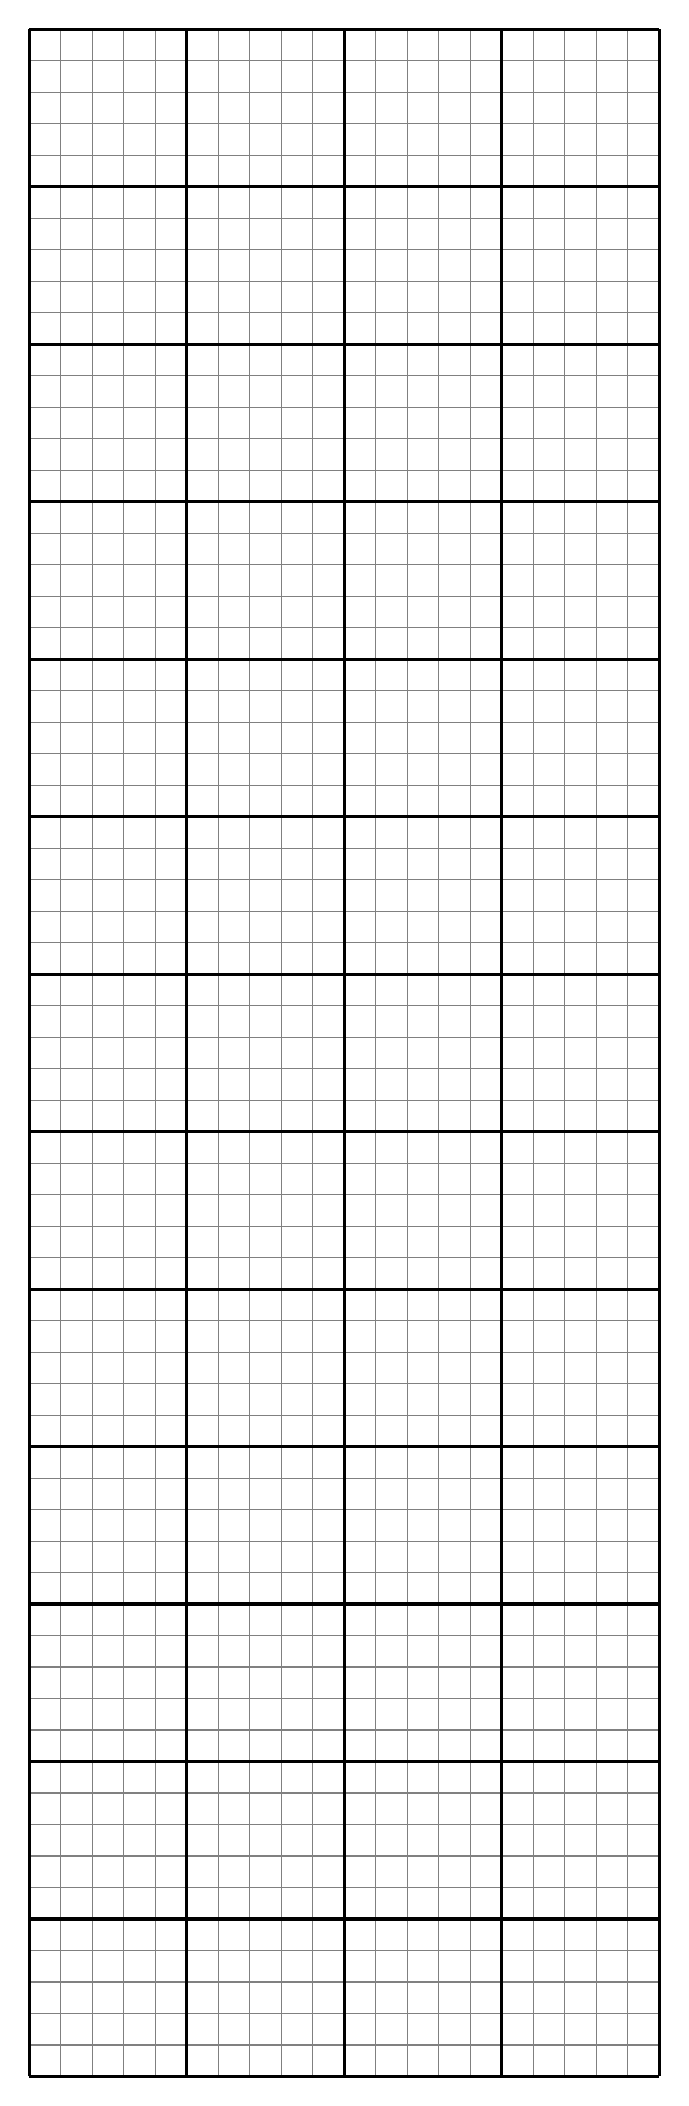
\begin{tikzpicture}[every node/.style={minimum size=1cm-\pgflinewidth, outer sep=10pt}, scale=2]
    \draw[step=0.2cm,color=gray] (0,0) grid (4,13);
    \draw[step=1cm,color=black,line width=0.4mm] (0,0) grid (4,13);
\end{tikzpicture}
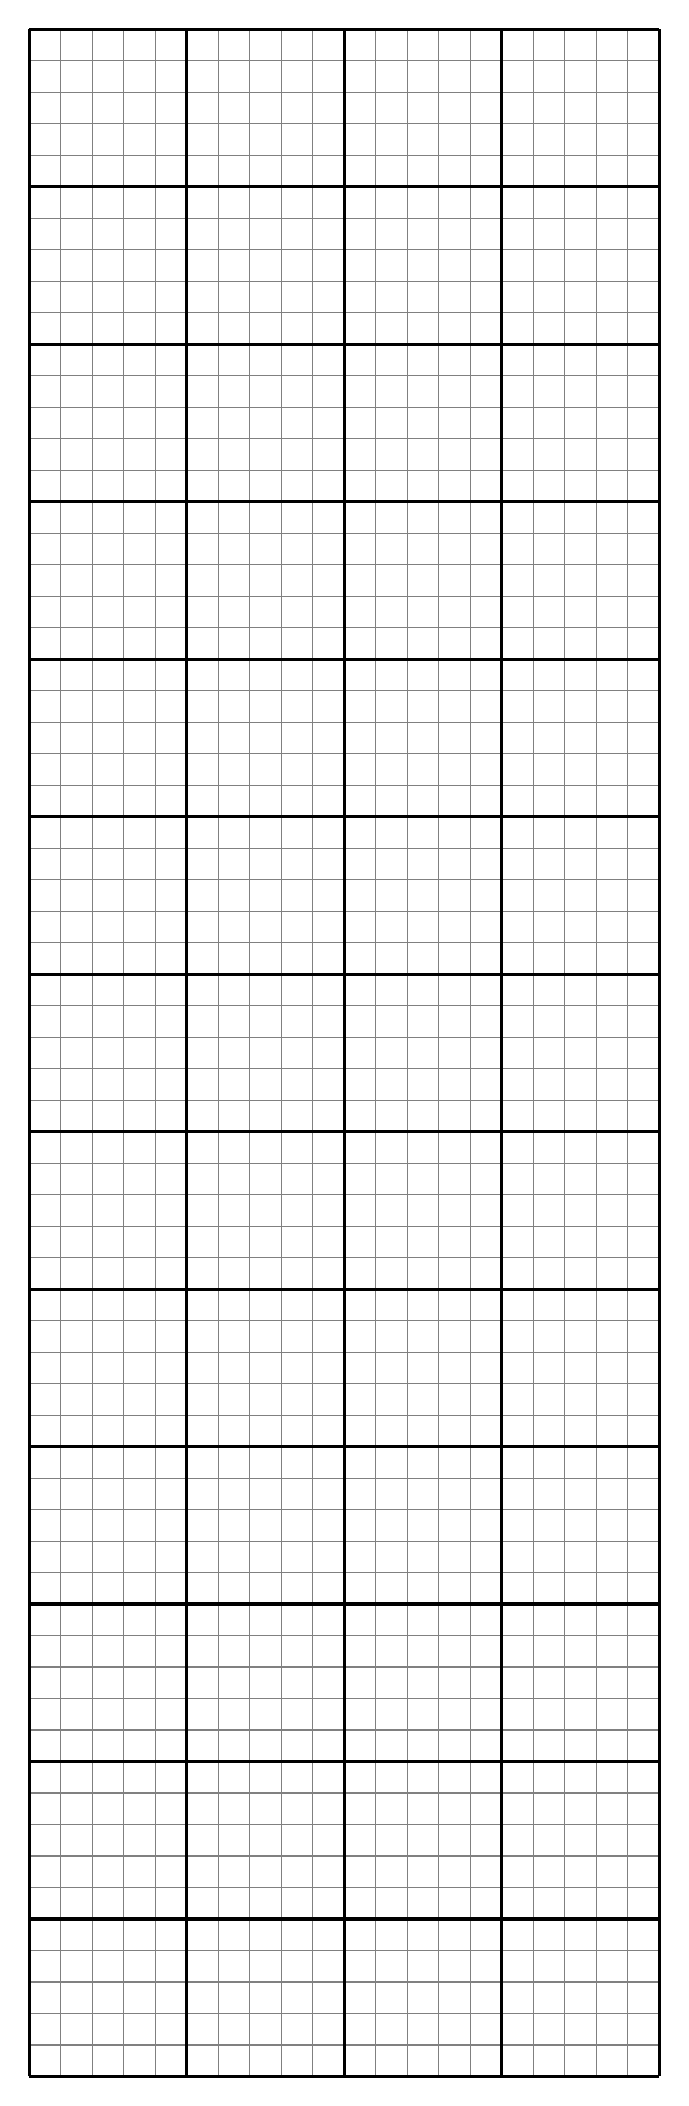
\begin{tikzpicture}[every node/.style={minimum size=1cm-\pgflinewidth, outer sep=10pt}, scale=2]
    \draw[step=0.2cm,color=gray] (0,0) grid (4,13);
    \draw[step=1cm,color=black,line width=0.4mm] (0,0) grid (4,13);
\end{tikzpicture}
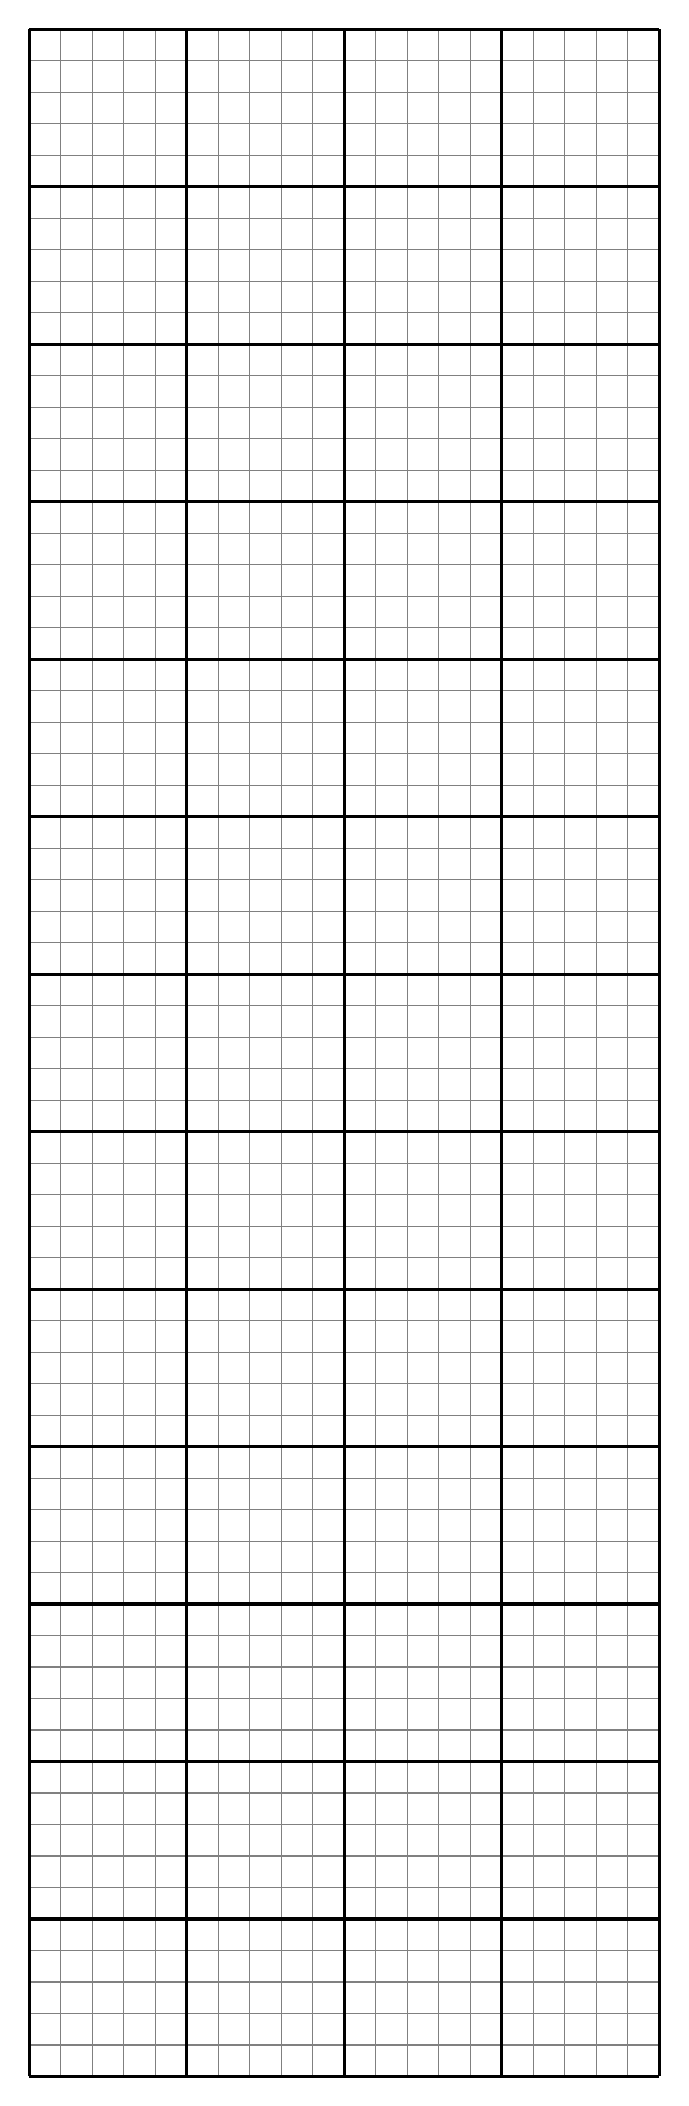
\begin{tikzpicture}[every node/.style={minimum size=1cm-\pgflinewidth, outer sep=10pt}, scale=2]
    \draw[step=0.2cm,color=gray] (0,0) grid (4,13);
    \draw[step=1cm,color=black,line width=0.4mm] (0,0) grid (4,13);
\end{tikzpicture}
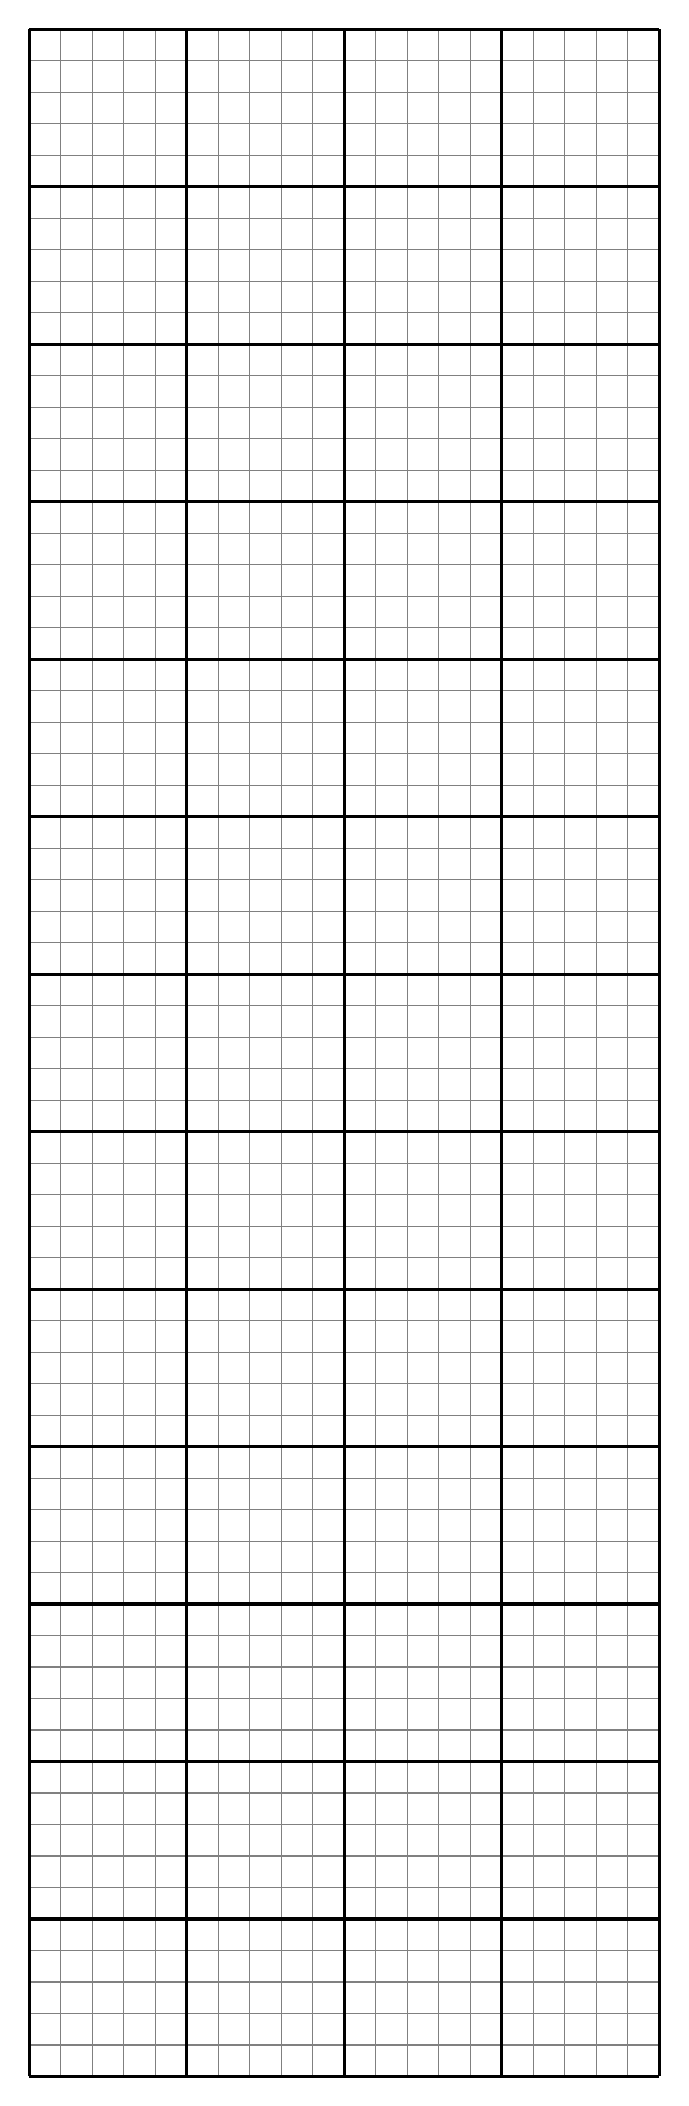
\begin{tikzpicture}[every node/.style={minimum size=1cm-\pgflinewidth, outer sep=10pt}, scale=2]
    \draw[step=0.2cm,color=gray] (0,0) grid (4,13);
    \draw[step=1cm,color=black,line width=0.4mm] (0,0) grid (4,13);
\end{tikzpicture}
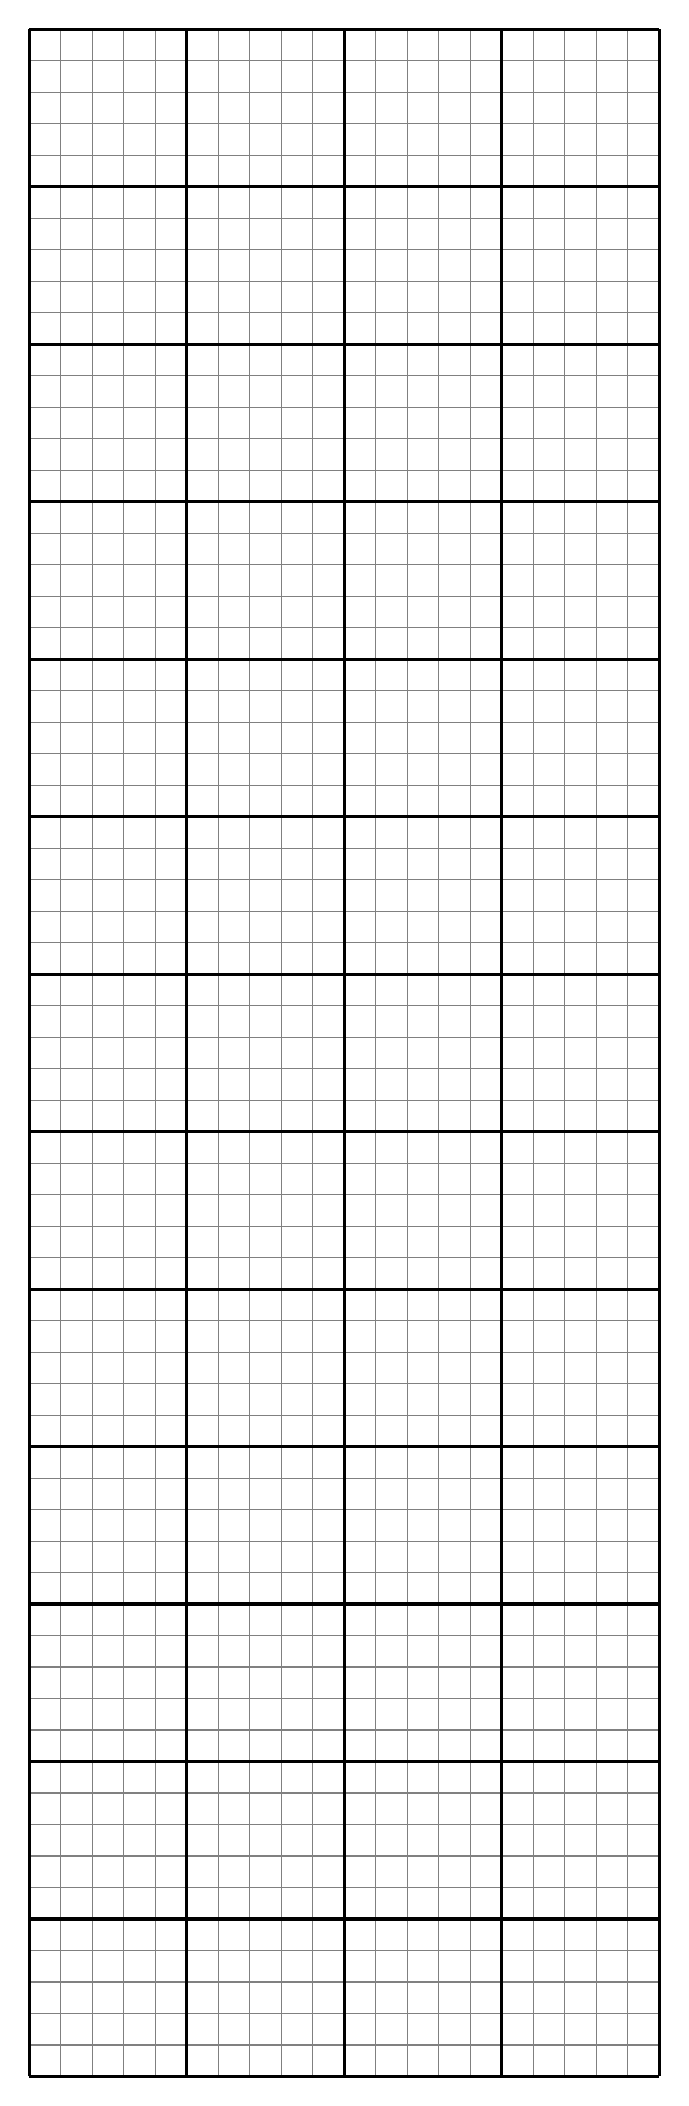
\begin{tikzpicture}[every node/.style={minimum size=1cm-\pgflinewidth, outer sep=10pt}, scale=2]
    \draw[step=0.2cm,color=gray] (0,0) grid (4,13);
    \draw[step=1cm,color=black,line width=0.4mm] (0,0) grid (4,13);
\end{tikzpicture}
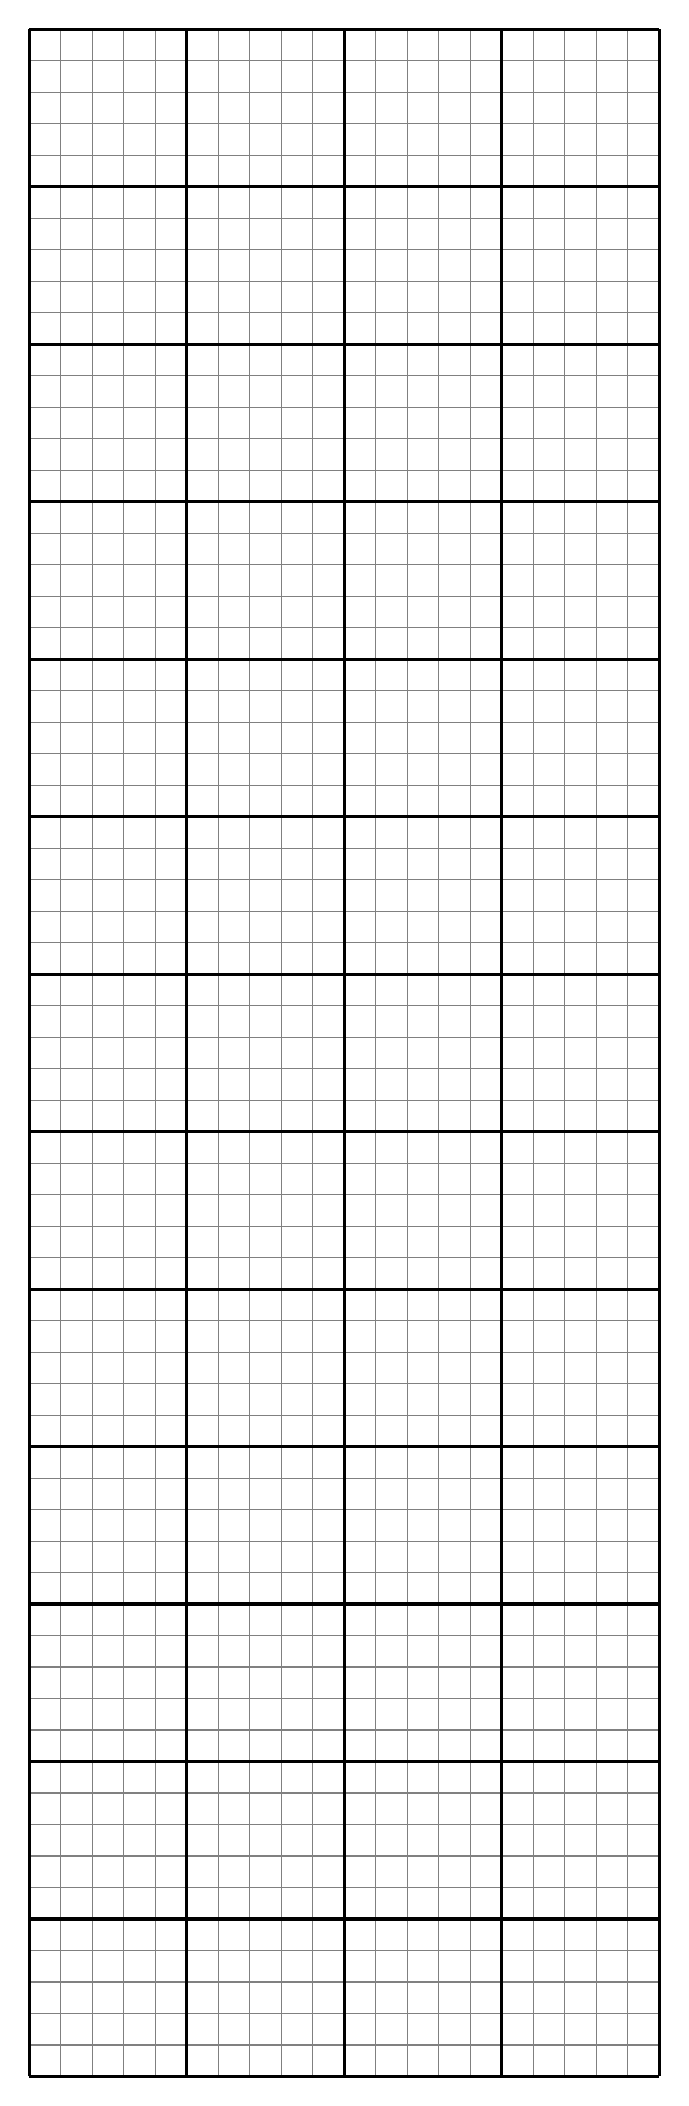
\begin{tikzpicture}[every node/.style={minimum size=1cm-\pgflinewidth, outer sep=10pt}, scale=2]
    \draw[step=0.2cm,color=gray] (0,0) grid (4,13);
    \draw[step=1cm,color=black,line width=0.4mm] (0,0) grid (4,13);
\end{tikzpicture}
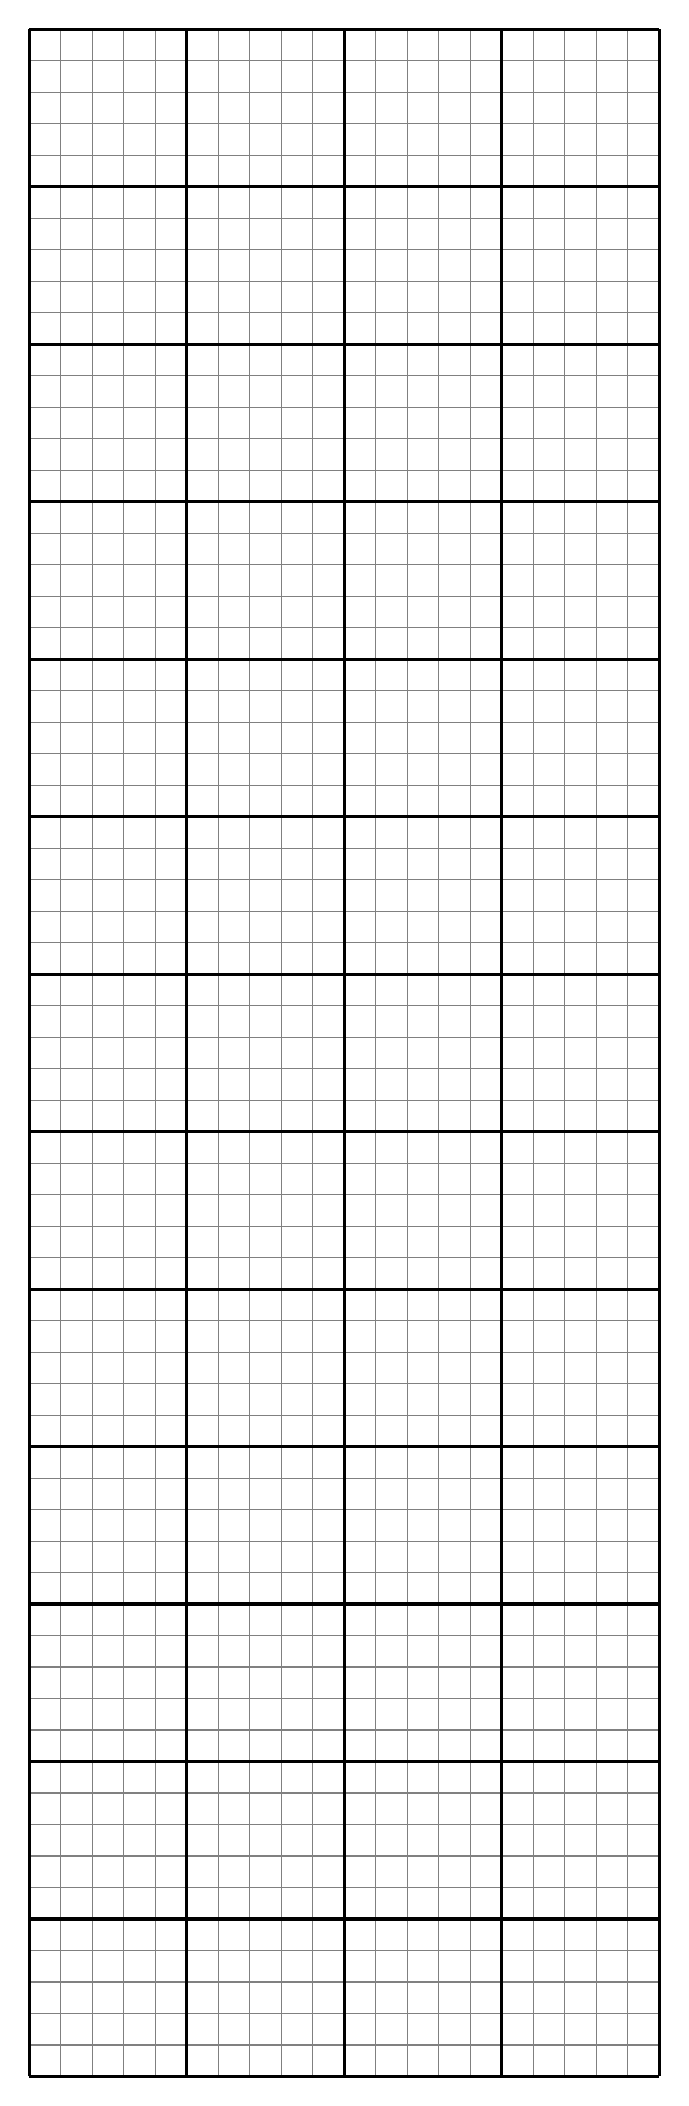
\begin{tikzpicture}[every node/.style={minimum size=1cm-\pgflinewidth, outer sep=10pt}, scale=2]
    \draw[step=0.2cm,color=gray] (0,0) grid (4,13);
    \draw[step=1cm,color=black,line width=0.4mm] (0,0) grid (4,13);
\end{tikzpicture}
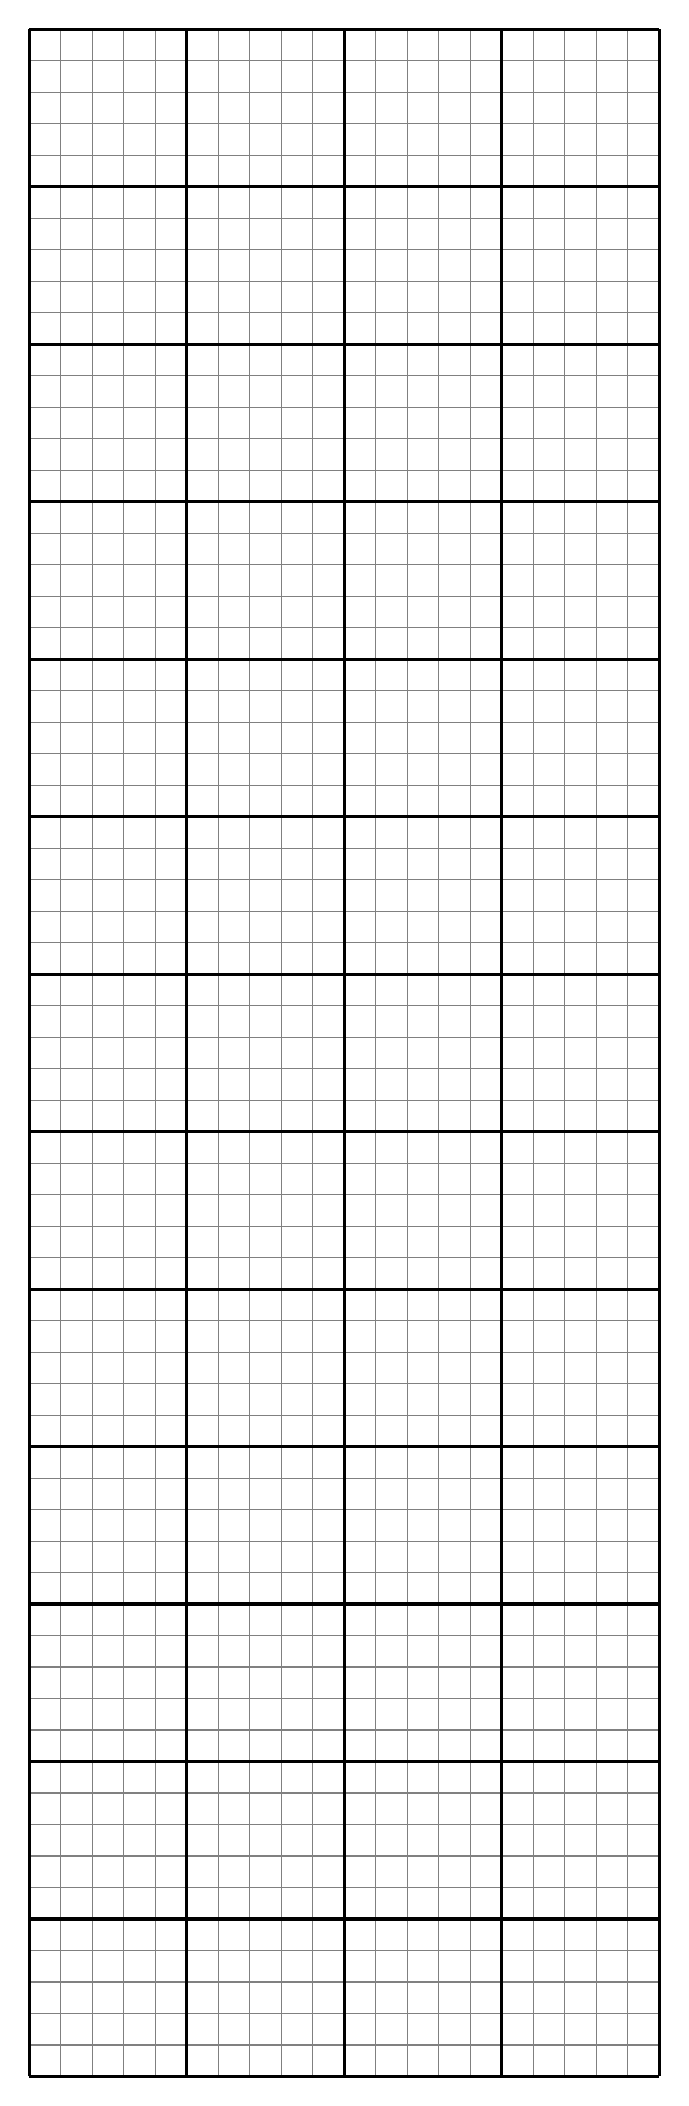
\begin{tikzpicture}[every node/.style={minimum size=1cm-\pgflinewidth, outer sep=10pt}, scale=2]
    \draw[step=0.2cm,color=gray] (0,0) grid (4,13);
    \draw[step=1cm,color=black,line width=0.4mm] (0,0) grid (4,13);
\end{tikzpicture}
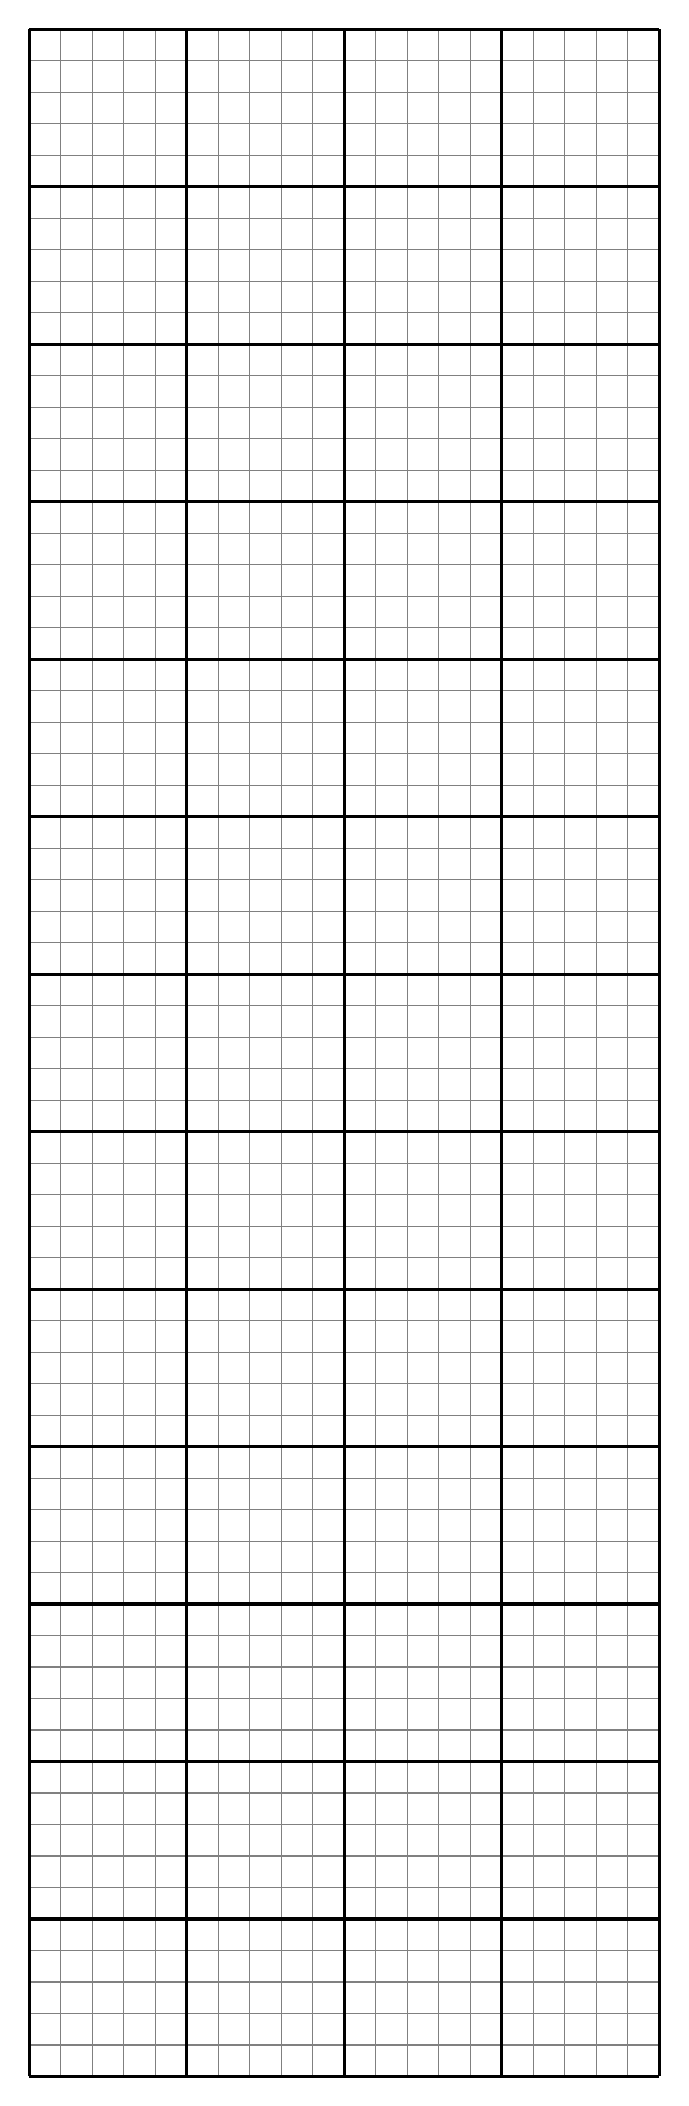
\begin{tikzpicture}[every node/.style={minimum size=1cm-\pgflinewidth, outer sep=10pt}, scale=2]
    \draw[step=0.2cm,color=gray] (0,0) grid (4,13);
    \draw[step=1cm,color=black,line width=0.4mm] (0,0) grid (4,13);
\end{tikzpicture}

\end{document}